\documentclass{article}

% if you need to pass options to natbib, use, e.g.:
% \PassOptionsToPackage{numbers, compress}{natbib}
% before loading nips_2017
%
% to avoid loading the natbib package, add option nonatbib:
% \usepackage[nonatbib]{nips_2017}

\usepackage{nips_2018}

% to compile a camera-ready version, add the [final] option, e.g.:
% \usepackage[final]{nips_2017}

\usepackage[utf8]{inputenc} % allow utf-8 input
\usepackage[T1]{fontenc}    % use 8-bit T1 fonts
\usepackage{hyperref}       % hyperlinks
\usepackage{url}            % simple URL typesetting
\usepackage{booktabs}       % professional-quality tables
\usepackage{amsfonts}       % blackboard math symbols
\usepackage{nicefrac}       % compact symbols for 1/2, etc.
\usepackage{microtype}      % microtypography
\usepackage{graphicx}

\title{Excitatory and suppressive features of auditory neurons in avian cortex}

% The \author macro works with any number of authors. There are two
% commands used to separate the names and addresses of multiple
% authors: \And and \AND.
%
% Using \And between authors leaves it to LaTeX to determine where to
% break the lines. Using \AND forces a line break at that point. So,
% if LaTeX puts 3 of 4 authors names on the first line, and the last
% on the second line, try using \AND instead of \And before the third
% author name.

\author{
  Timothy Tadros\\
  Department of Neurosciences\\
  University of California, San Diego\\
  La Jolla, CA 92037 \\
  \texttt{tttadros@ucsd.edu} \\
  \And
  Tatyana O. Sharpee\\
  Computational Neurobiology Labratory\\
  Salk Institute for Biological Studies\\
  La Jolla, CA 92037\\
  \texttt{sharpee@salk.edu}\\
}

\begin{document}
% \nipsfinalcopy is no longer used

\maketitle

\begin{abstract}
  The ability to process auditory signals and ignore the noise is an influential reason why animals depend on acoustic signals for communication and survival. Previous work on auditory receptive fields has uncovered many different types of auditory neurons: broadband neurons are tuned to signals across all frequency ranges but only at a specific time. Narrow-band neurons respond only to signals in very specific time and frequency windows. While there has been a lot of work in describing receptive fields of different auditory processing regions, little has been done to connect this work with computational theories of auditory processing. Here we analyze responses of auditory neurons in songbirds in four different regions in auditory cortex to various songs and find various principles that explain how auditory processing is organized. First, there are more suppressive features than excitatory features further downstream, indicating more feature selectivity as the signal is transmitted through cortex. Second, quadrature pairs and cross-orientation suppression, etc. This principles is consistent with the time-dilation theory of auditory processing, etc...
\end{abstract}

\section{Introduction}

Auditory processing utilizes a number of complex and poorly understood transformations as sound is transduced from the midbrain (mld) up through the thalamus (nucleus oviodalis (OV)) and onto auditory cortex (Field L and CM) \cite{ondracek2013advances}. While previous work in songbirds has looked at the number of broadband and narrowband neurons in each region of auditory processing illustrating a possible function or set of functions for each region \cite{woolley2009functional}-\cite{amin2010role}, it is still poorly understood how the sum of the parts can give rise to complex auditory behavior that aids in survival, such as identifying a stranger vs. a relative, a mate vs. a non-mate, etc.. One important question is how the combination of excitatory and suppressive features and the organization of receptive fields with different features can give rise to complex sound recognition and interpretation. For example, neurons in Field L are thought to receive input from an excitatory and inhibitory neuron and process these inputs nonlinearly \cite{nagel2008organizing}. This nonlinearity may give rise to intensity-dependent receptive fields, which enables the bird to encode and distinguish near and far songs.

To address these questions of how the receptive fields of auditory neurons are organized, we utilized the statistical model of maximum likelihood estimation to determine the receptive fields of auditory neurons. After computing these receptive fields, we fit them as a linear combination of gammatones and gaussian filters in order to analyze the features of these receptive fields. After performing this modelling, we conclude that (1) suppression is increased as a signal is transduced along the auditory pathway, (2) auditory signalling is composed primarily of broadband and narrowband receptive fields with little intermediate receptive fields, (3) ...... Overall, these findings show that ...

\section{Quadratic model}

Using a published dataset of neural responses in songbirds to various songs on the CRCNS data sharing website, we sought to build a model that maps the input stimuli to the collected neural responses with high probability. The dataset included neural responses in songbirds from various regions in auditory cortex (mld, field L, OV, and CM) to different song recordings. Treating each song as a $d-$dimensional vector over time $x$, we computed the predicited response $Y'$ of the model as follows:
$$
Y = \sigma(a + \mathbf{h}\cdot x + x\mathbf{J}x^T)
$$ where $\sigma$ is the sigmoidal function
$$\sigma(x) = \frac{1}{1+e^{-x}}.$$ Here $h$ is a $d-$dimensional filter that illustrate the linear features of the model. $\mathbf{J}$ is a $d\times d$-dimensional matrix comprised of the quadratic features that best fit the model. $a$ is simply the bias of the neuron. All of the parameters $a, h, \mathbf{J}$ were fit by minimizing the negative log-likelihood of the model.

We divided the training data into fourths. Three-fourths of the data were used to calculate the gradient and the other fourth was used as a validation set to determine convergence. We ran 4-fold cross validation using a different fourth of the training data as a holdout set and averaged each parameter over the four trials to control for variability in the optimization process. To test the model, we held out recordings for each neuron and then tested our model on these held out recordings.

\paragraph{Receptive fields}

In order to compute the basis of pertinent dimensions of $\mathbf{J}$ along which the neuron responds most strongly, we performed eigendecomposition of $\mathbf{J}$ to get the eigenvectors and eigenvalues. This resulted in a number of eigenvectors and eigenvalues, only a few of which were significant. %% how is significance determined
After significance testing, only a few eigenvectors remained for each neuron. These eigenvectors illustrate the dimensions along which a neuron responds most maximally to and thus can be considered the receptive fields of the neuron. Eigenvectors with positive eigenvalues are excitatory features and those with negative eigenvalues are suppressive features. An example of eigendecomposition is shown in %%figure.

\paragraph{Excitatory and suppressive features}


\section{Linear combination of gammatones}
\paragraph{Methods}
Gammatones are widely used as auditory filters. In order to model the receptive fields computed above, we attempt to build J using a linear combination of gammatones. A gammatone is described by the following equation:$$g(t) = a(t-t_0)^{n-1}e^{-2\pi b(t-t_0)}\cos({2\pi f (t-t_0) + \phi}),
$$ where $a$ controls the amplitude, $t_0$ controls the onset time, $n$ controls the filter order, $b$ controls the decay rate, $f$ controls the central frequency, and $\phi$ controls the phase. Since, this is only a function of time, we take the outer product of $g(t)$ and a Gaussian filter along the frequency dimension, with central frequency $f_0$ and standard deviation $\sigma$ to get a 2-d dimensional receptive field, denoted as $S$. Example gammatones are shown in figure. %%figure of example gammatones 

With a set of gammatones we can approximate $\mathbf{J}$ as $$\mathbf{J'} = \sum_{i}{SS^T}.$$ We ignore any weights as the $S$ matrices are normalized when performing the fit. We choose to fit the onset time, filter order and decay rate of the gammatone, as well as the central frequency and standard deviation of the gaussian using differential evolution. All other paramaters are either redundant because normalization is performed ($a$) or irrelevant to the problem we are interested in ($\phi$).  We seek to minimize the mean difference between $\mathbf{J}$ as computed using the quadratic model and the new $\mathbf{J'}$. The excitatory and suppressive parts of $\mathbf{J}$ were fit seperately and only the significant eigenvectors are taken into consideration. The exact approach we took to solve the differential evolution problem can be read about in %%cite ryans paper.




\paragraph{Results}

\paragraph{Analysis of different auditory regions}
\paragraph{Cross-order suppression}
\paragraph{Quadrature pairs}

\begin{figure}
  \centering
  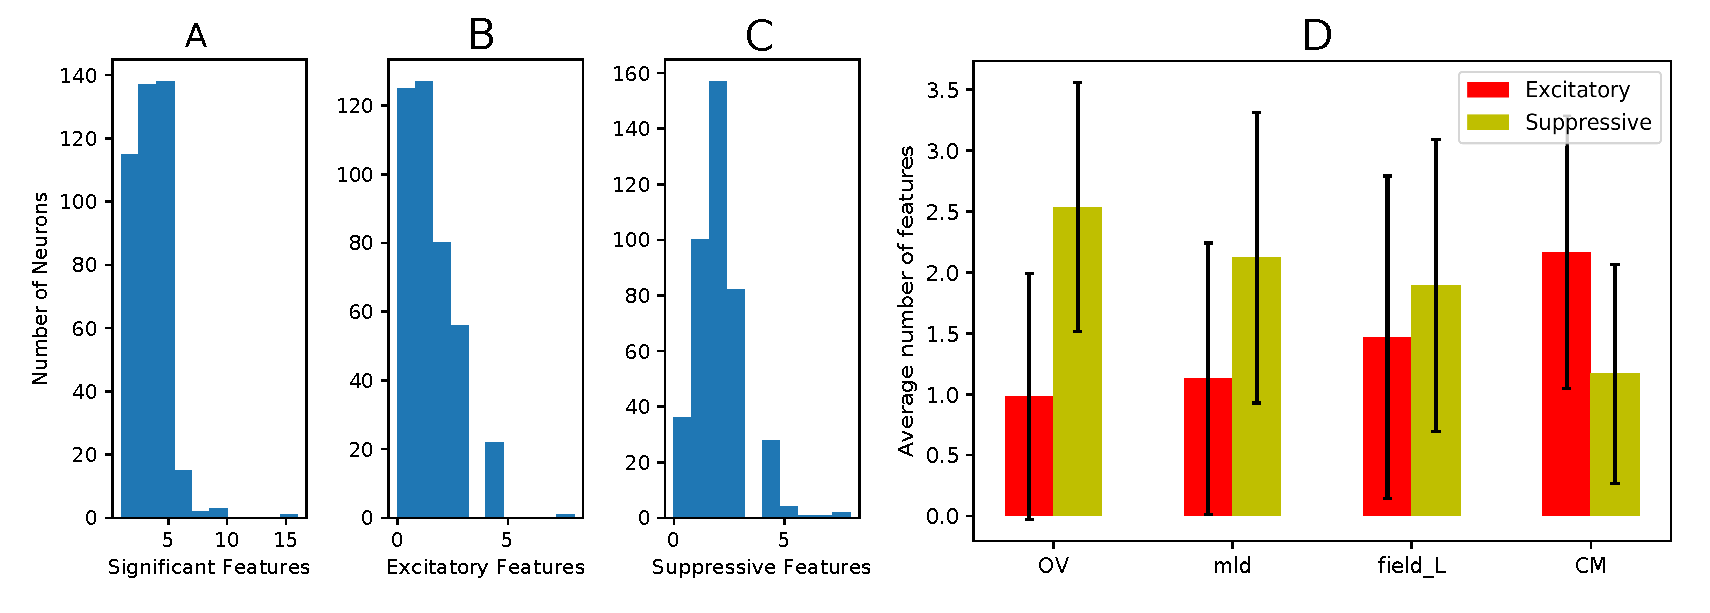
\includegraphics[width=1.0\linewidth]{Figures/Figure1.eps}
  \caption{The distribution of the number of significant, excitatory, and suppressive features computed through the convolutional model. (A) The total number of significant dimensions of J. (B) The number of significant dimensions with positive eigenvalues. (C) The number of significant dimensions with negative eigenvalues. (D) Average number of excitatory and suppressive features for each region in auditory cortex.}
\end{figure}

\begin{figure}
  \centering
  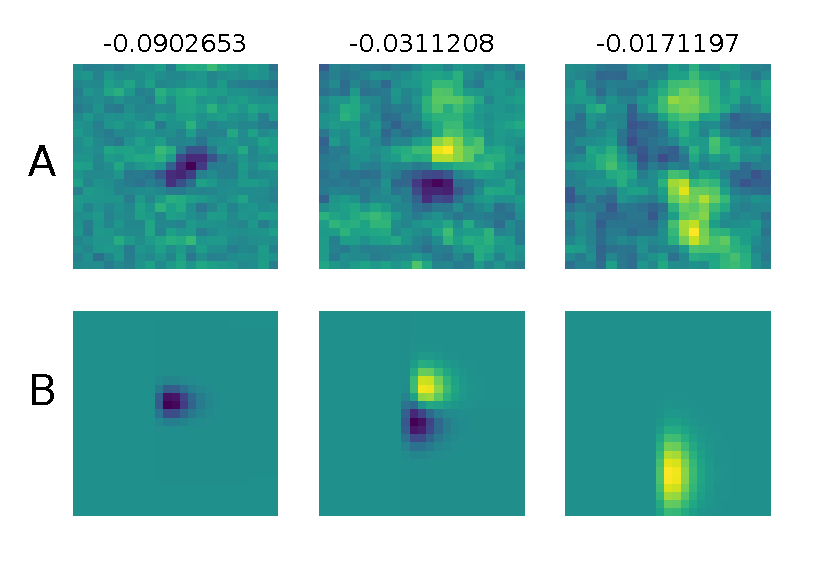
\includegraphics[width=1.0\linewidth]{Figures/Figure2.eps}
  \caption{Example auditory receptive field with 3 suppressive features. The neuron is $glb5656_2$ in the ovoidalis. (A) Receptive fields computed from the quadratic model. There are 3 significant dimensions for this neuron and they are all suppressive (eigenvalues listed above the receptive field. (B) Gammatones fit to the receptive fields above. Parameters were selected manually to illustrate the process of fitting a linear combination of gammatones to the J matrix.}
\end{figure}

\begin{figure}
  \centering
  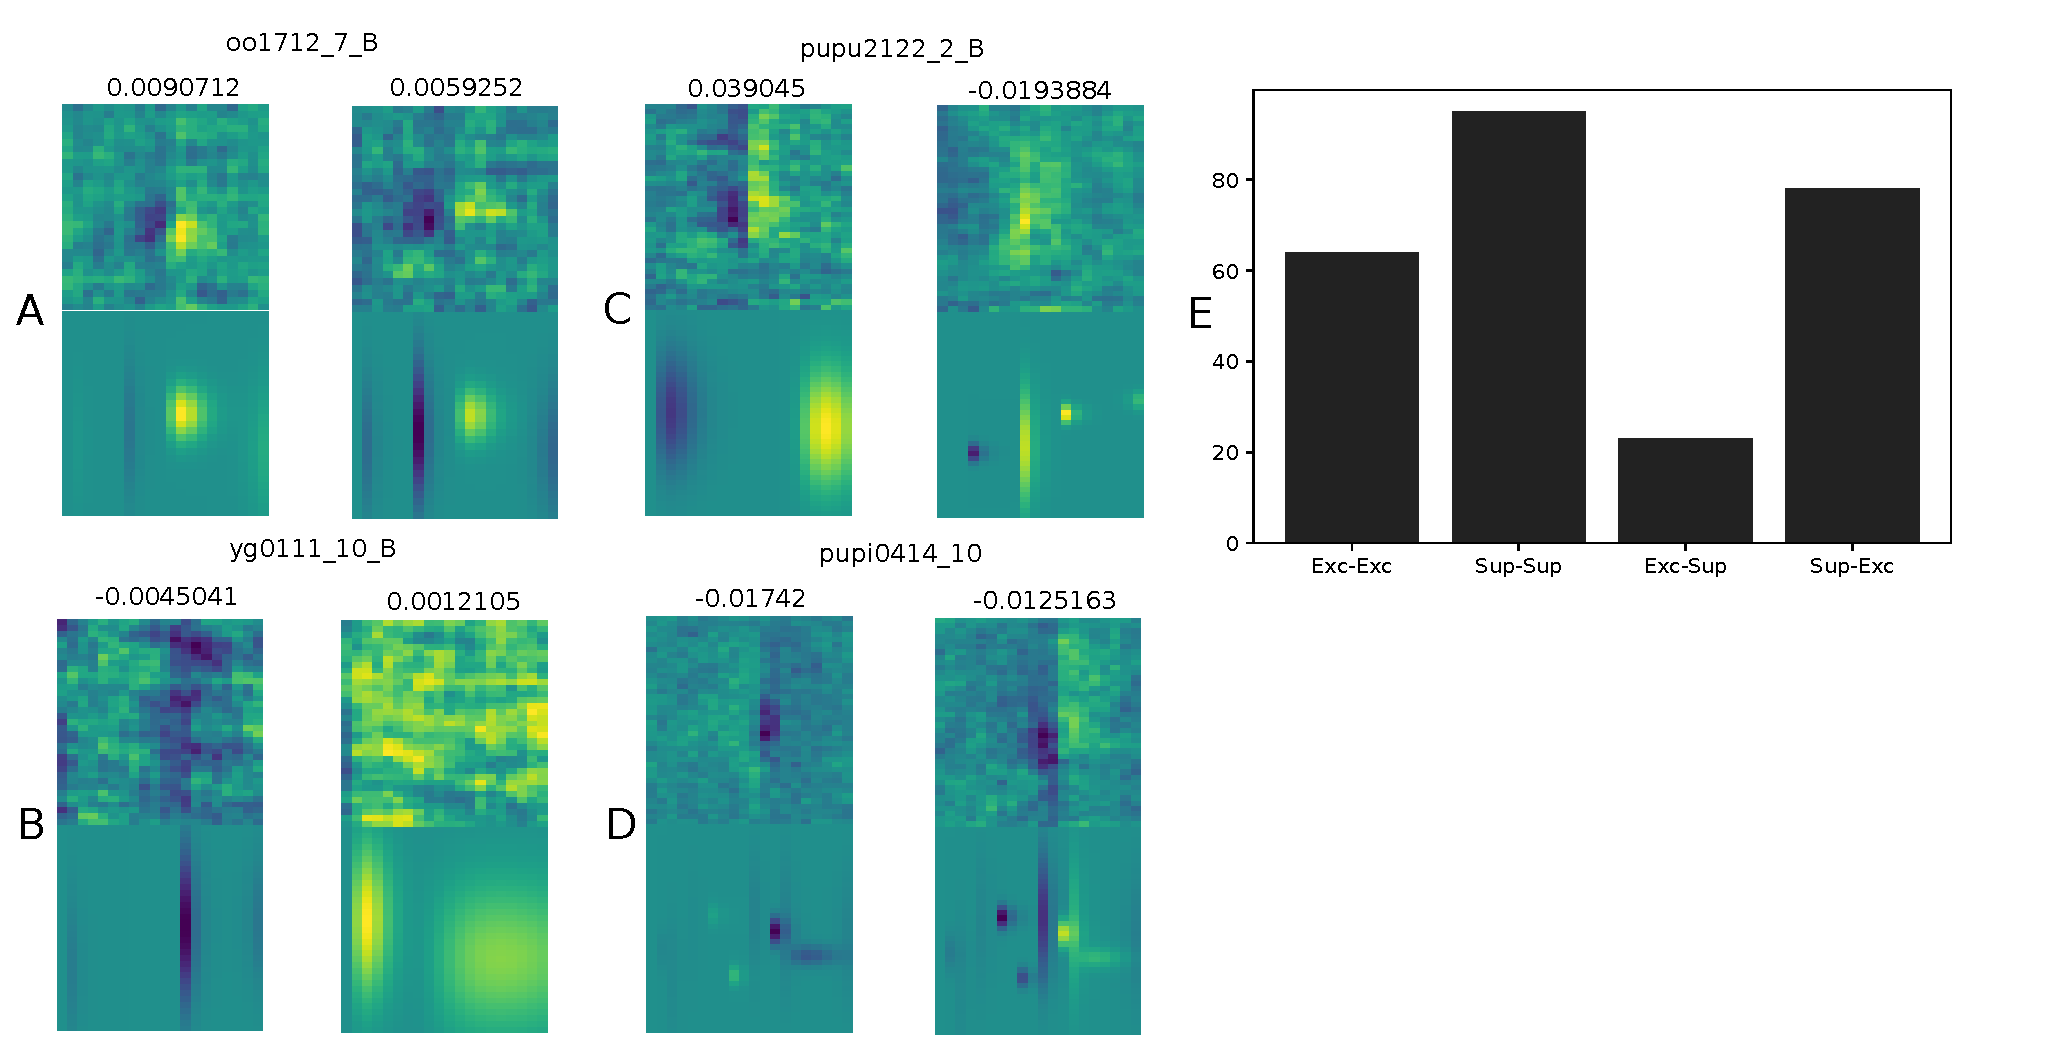
\includegraphics[width=1.0\linewidth]{Figures/Figure3.eps}
  \caption{Using differential evolution to fit gammatones to the J kernel from the quadratic model. (A)-(D) show example fits for the two most significant dimensions of J for 4 categories of neurons: (A) excitatory-excitatory, (B) suppressive-excitatory, (C) excitatory-suppressive, and (D) suppressive-suppressive. The top row of each of these panels is the receptive field for the neuron computed as the eigenvectors of the J kernel. The bottom row is the example fit computed through differential evolution. The numbers are the eigenvalues for each dimension. (E) illustrates the number of neurons in each of the 4 categories.}
\end{figure}

\section{Discussion}

\bibliographystyle{unsrt}
\bibliography{references}


%\section*{References}
%\medskip

%\small

%[1] Ondracek, J. M.\  \& Hahnloser, R. H.\ (2013). Advances in understanding the auditory brain of %songbirds. In {Insights from Comparative Hearing Research} pp.\ 347-388. Springer, New York, NY.

\end{document}